In this chapter, we regard an example solution for event stream analytics. While this is only one specific incarnation and many different designs are possible, it highlights important aspects that every solution needs to consider. The solution is independent of the use case presented in the next chapter and therefore applicable to many scenarios. In any case, \cite{Kleppmann.2017} is a good foundation for designing distributed data processing solutions.





\section{Requirements}
The goal of the solution is to ingest data from an external stream source, process the stream to produce insights, and visualize those insights in real time. Arriving at those insights requires stateful processing in the correct order that goes beyond record-by-record transformations. Additionally, we want to see results in real time regardless of the data volume. This leads us to the four requirements that have guided us through the past two chapters:
\begin{itemize}
	\item Correctness: results should be guaranteed to be correct through exactly-once event-time-order processing even if events arrive out of order and faults occur
	\item Fault tolerance: the solution should guarantee consistent results and preserve state during faults without heavy recomputations
	\item Low latency: results based on an ingested event should become available for visualization in (near) real time (a latency of a few seconds is acceptable/inevitable, depending on the job)
	\item Scalability: the solution should be able handle large volumes of data without performance degradation
\end{itemize}
Correctness and fault tolerance go hand in hand, but are in tension with low latency and scalability. Providing real-time results of computations at high volume requires a distributed stream processing platform that spans across nodes, but keeping consistent distributed state without impacting performance severely is challenging. The challenge becomes easier when using fast solid state drives, large memory pools and nodes with many CPU cores. We will disregard the cost factor in this design since we approach the problem from a technical perspective. However, the combination of Kafka and Flink for stream transport and stream processing can fulfill all of the four requirements even on inexpensive commodity hardware through efficient designs and implementations, and allows us to build jobs on top while taking care of the execution.





\section{Architecture}
The components and stream flow of our architecture are shown in figure~\ref{fig:solution-architecture}. All components run on separate clusters of nodes but shared nodes are possible as well. Kafka sits at the core to provide stream transport and storage while decoupling producers and consumers. Having Kafka act as a durable buffer enables replay for fault tolerance, but also prevents consumers from being overwhelmed by faster producers and allows producers not to be held up by failing consumers. Additionally, consumers can flexibly be added or start reading at different offsets without affecting the producer. While every stream only has a single consumer in our architecture, more consumers could be added, for example for monitoring, data warehousing or event-driven applications. This kind of centralized platform can democratize data and allow seamless integration and streamlined dataflow between different teams in an organization. The Zookeeper cluster required for Kafka broker coordination and Flink high availability runs on the same nodes as the Kafka cluster, but can easily be extracted into a separate cluster for isolation in case of faults.

We define all infrastructure (nodes, network, storage) as code using Terraform\footnote{\url{https://www.terraform.io/}}, which provisions the resources on AWS. We then import the data into Ansible\footnote{\url{https://www.ansible.com/}} using a custom dynamic inventory script to deploy the platforms and components. This fully automated deployment allows us to quickly set up and tear down everything and treat our infrastructure as immutable. This means that we do not change existing infrastructure but always make a clean and consistent deployment. Any data is stored externally so no data is lost in this process. However, we have not done extensive online updates yet, so the deployment approach might need to be adjusted for large-scale production situations.

\begin{figure}
	\centering
	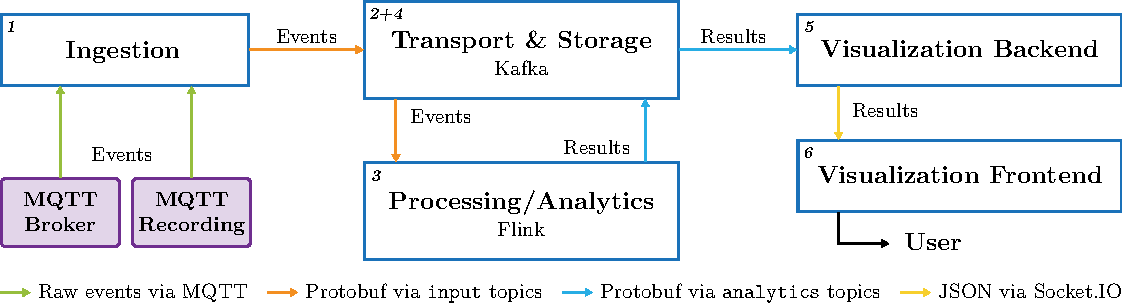
\includegraphics[width=\textwidth]{solution_architecture}
	\caption[Solution architecture]{Solution architecture: streams flow from sources through ingestion and processing to visualization, this order is also denoted by the numberss.}
	\label{fig:solution-architecture}
\end{figure}

Streams are not initially created within our solution but ingested from an external source. This source can be anything from database change captures over message queues to arbitrary event sources. The ingestion component is responsible for capturing these external events, filter and transform them, and write them to the appropriate Kafka topic. Therefore it basically acts as connector to the outside world. Analytics jobs running in the Flink cluster of the processing component consume these input streams and write their analytics results back into Kafka. The visualization component consumes the results streams in the backend and forwards them to the frontend, where they are displayed in real time in a format appropriate for the use case. This could, for example, be a dashboard for monitoring or a map for geospatial data. Having the visualization consume a stream is different from most traditional user interfaces which query a database or web service. We are deliberately using an end-to-end streaming design to embrace the continuous nature of our data.



\subsection{Transport and Storage}
With the current set of components, there are two types of Kafka topics. Topics prefixed with \texttt{input} originate in the ingestion component, and topics starting with \texttt{analytics} are produced by the processing component. A clear and consistent naming scheme helps when adding more topics and producers but can be chosen freely. The number of partitions needs to be chosen based on the expected data volume, with random partitioning for even distribution if possible. This does not retain the order of incoming events but we rely on Flink for processing in the correct order. We use a replication factor of 3 for each topic since this provides a good balance between fault tolerance and performance. The number of total partitions determines the required cluster size. We use a short retention period which is higher than the Flink checkpointing period since we only use retention for fault tolerance, not replays from a much earlier point in time. Note that the disk size requirements increase proportionally to the data volume and retention period. We configure our cluster to be accessible from the outside from certain address ranges. While this is not recommended for production setups, it allows developers to run certain components on their local computer during development or peek into topics for debugging.

We have one topic per event type, with all records having a common schema. We use \gls{protobuf} for schema specification since it has support for many languages, flexible records and schema evolution. There are two serialization modes. The binary mode creates compact messages, while the JSON mode creates human-readable messages suitable for debugging. Switching between these modes is simple and allows, for example, to use JSON during development but binary for production. Every record, whether input or analytics result, has the schema shown in listing~\ref{lst:solution-protobuf-event-schema}. We refer to the common schema defined in \protobufinline/Event/ as base event. The \protobufinline/event_timestamp/ may contain the actual time the event occurred if the external source provides such a timestamp, or the end of the event time window for analytics results. The \protobufinline/ingestion_timestamp/ is the local system time in the ingestion and processing components before handing over the record to Kafka. The \protobufinline/details/ are an arbitrary nested \gls{protobuf} message which is specific to the event type. The \protobufinline/Any/ attribute type stores the nested type name and actual object to be able to deserialize the event with type safety. The structure of the type can be looked up in a type registry that is compiled into the components, but a central schema registry such as the one bundled with Confluent becomes indispensable when the number of producers and consumers grows.

\begin{listing}
\inputminted{protobuf}{code/solution_protobuf_event_schema.proto}
\caption{Common Protocol Buffers schema for all events}
\label{lst:solution-protobuf-event-schema}
\end{listing}



\subsection{Ingestion}
All input streams originate at an external source and therefore need to be integrated into the solution first. This is the task of the ingestion component. Incoming events are first filtered so only relevant ones are ingested into the system. Then they are converted to the specific \gls{protobuf} schema of the event type by selecting attributes and casting them to the right data types. Together with an extracted event timestamp, they are wrapped in the common event schema and produced to the appropriate Kafka topic prefixed with \texttt{input}. The current implementation of the ingestion component only supports a single node and no fault tolerance, but it can be extended in the future to run in a distributed fashion by dividing the input streams between multiple nodes. For example, each node could be assigned a mutually exclusive subset of source partitions for ingestion. Note that multiple nodes might require distributed coordination in case shared state is required, in which case the implementation of the partitioning is not as straigtforward anymore. Another alternative is to use an existing tool like Kafka Connect instead of a custom implementation if only simple transformations need to be done.

Our implementation provides flexibility through two base abstractions that work together as shown in listing~\ref{lst:solution-ingestion-abtractions}\footnote{We use Python-inspired pseudocode for all code listings in this thesis for brevity.}. A \pythoninline/Connector/ connects to the external source to receive the raw event stream. Every raw event is processed by the \pythoninline/Processor/, which determines if an event should be filtered out and therefore not be ingested, or extracts the timestamp and event details with the correct \gls{protobuf} schema. These are then wrapped in a base event where the ingestion timestamp is added, serialized to the binary or JSON \gls{protobuf} wire format, and ingested into the appropriate Kafka topic. Multiple connector can be run in parallel.

\begin{listing}[t]
	\inputminted{python}{code/solution_ingestion_abstractions.py}
	\caption{Interaction between connectors and processors}
	\label{lst:solution-ingestion-abtractions}
\end{listing}

The \pythoninline/Connector/ and \pythoninline/Processor/ abstractions based on a common interface allow easy extension of the ingestion component for a wide range of different source types. We provide connectors for two types. The first connector subscribes to topics on an MQTT\footnote{MQTT is a publish--subscribe protocol commonly found in IoT applications. A central broker routes events from clients who publish them to clients which have subscribed certain topics of events. Topics are often structured hierarchically, but the topic format can be chosen at will.} broker. The topics to subscribe to are determined by the processor. The second connector replays a recording of MQTT events captured with a custom tool. The recording is streamed from S3 while preserving the original timing between events. The processor can also modify the event, for example to adjust the event timestamp to the current time. Replaying previous recordings is useful for repeatability of evaluations. Decoupling the event source and pre-processing using the two abstractions allows us to use the same processor for multiple connectors.



\subsection{Processing}
The actual event stream analytics happen in the processing component, which is a Flink session cluster on which all jobs run. All jobs consume the input topics for the events they require, and produce their results to a job-specific topic prefixed with \texttt{analytics}. This allows downstream consumers to receive only the analytics they are interested in. The cluster consists of 3 job managers for high availability, but the number of task managers is determined by the number of jobs, their parallelism (the number of task slots required can be equal to the highest parallelism with slot sharing), and how many task slots each task manager offers (usually equal to the number of CPU cores). For example, 5 jobs where the operator with the higest parallelism has a parallelism of 20 requires 25 task manager nodes when each node has 4 cores and slot sharing is enabled. The parallelism needs to be adjusted to the expected throughput and the number of Kafka partitions. If there is only a single partition, the whole topic is consumed from and redistributed by a single task, even if the configured parallelism is higher. Note that increasing the number of nodes increases the overhead of shuffling after \texttt{keyBy} operations. The capacity planning depends on many factors like state size and backends bit also chaining and slow sharing, therefore we cannot give recommendations for the actual cluster size. \cite{Metzger.2018} shows rough calculations for the required network capacity.

All jobs are written in Java and extended a common base class. This base class handles the setup of checkpointing as well as event-time processing and exactly-once processing by default. However, at-least-once processing might be required for some ultra-low latency applications. The checkpointing frequency affects the required topic retention period and the recomputation effort in case of failures. However, if not many failures are expected, it can make sense to increase the delay between checkpoints. The base class also configures Kafka bootstrap servers and consumer groups, and provides methods for working with Kafka topics. Dataflow graph sources can be defined by the topic and expected event type, while the base class sets up the serialization and correct watermarking and event timestamp extraction from the base event. While we normally use the actual event timestamp, it would also be possible to assign the ingestion timestamp as event timestamp in this step to order events by the time they arrive at the ingestion component. Dataflow graph sinks can be defined by the job-specific topic, and another method handles the creation of the base event with the correct timestamps and details. Creating accurate heuristic watermarks is very hard. Therefore we use the bounded-out-of-orderness strategy based on the expected delay, which can for example be determined using offline analysis of the distribution of event-time skew. Once the distribution is known, a percentile watermark can be created with the threshold set to balance latency and completeness. If the watermark underestimates the event-time skew, many records are marked as late which increases computation effort when late triggers are enabled. Watermarks are emitted periodically every \SI{200}{\milli\second}, which is a good tradeoff between latency and computation effort, since most watermarks trigger downstream computations like window evaluations. In general, watermark boundedness and allowedness need to be configured to balance correctness/completeness, latency and cost/resource requirements. We do not guarantee end-to-end exactly-once processing in our solution, since that would require an idempotent or transactional sink. While Kafka supports transactions, the Kafka client used in the visualization component does not, therefore results might be produced with at-least-once semantics. However, exactly-once can be easily enabled once the client adds transaction support. Then the checkpointing frequency needs to be increased since transactions are only committed once the checkpoint was completed successfully.

We use RocksDB as state backend, which is recommended for production environments and supports large state. However, state size should be kept reasonably small since it influences checkpointing time and resource requirements. This especially applies to operations which must retain many records like windows or pattern matching. These are some optimizations to minimize state size:
\begin{itemize}
	\item Since a record is copied for every window it is assigned to, use longer evaluation periods when using large sliding windows. For example, an hourly sliding window evaluated every second would result in 3600 copies of every record. If the evaluation period is decreased to every \SI{10}{\second}, the number of copies is reduced by a factor of 10.
	\item If the window transformation supports eager aggregation (like summing or averaging), state size can be reduced significantly because records are collapsed into a single intermediate result instead of having to retain all records until evaluation. Therefore, use \javainline/AggregationFunction/ and \javainline/FoldFunction/ instead of \javainline/ProcessWindowFunction/ if possible.
	\item While there is only one active tumbling window at any point when using processing time, multiple tumbling windows can be active simultaneously when defined in event time. With a high bounded-out-of-orderness and allowed lateness, windows and records need to be retained much longer. While changing the watermark is usually not sensible since it affects correctness, keeping the allowed lateness low allows records to be garbage-collected earlier.
	\item Only send relevant parts of the record to downstream tasks to reduce serialization and network overhead as well as state size. For example, if only two attributes of a protobuf event are needed, map the incoming event to a two-tuple early in the dataflow.
\end{itemize}



\subsection{Visualization}
The visualization component is the only one with which end users interact. This component consists of two parts. The backend consumes the analytics result topics and forwards forwards them to the frontend using Socket.IO (a library for client--server communication transparently using WebSockets or HTTP), where the results are displayed in real-time in a format appropriate for the analytics. There are two technical reasons for not connecting the frontend directly to Kafka. First, the frontend needs to be written in JavaScript, and there is currently no JavaScript library to connect to Kafka from the browser. Secondly, the protobuf type registry would need to be part of the frontend for deserialization. Therefore, we deserialize the analytics result protobuf records in the backend and send plain JSON strings to the frontend. While this does not maintain the order of the ordered topic partitions, the order usually does not matter for display. Currently, the frontend receives all analytics results but only displays those that the user has selected, so there is no communication from the frontend to the backend. Moving this responsibility of determining the data display to the frontend allows us to support multiple frontend users without extra effort.

While the backend is very simple and effectively only forwards events, the frontend has the challenge of invalidating events. When aggregating over keyed windows, windows are only created when there are actually events for that key. If a key creates windows for multiple subsequent windows, the frontend can simply display those results as updates to the previous results. However, once a key disappears (for example a user ends his session), no updated results are produced for that key. In these situations, the frontend needs to decide when to stop displaying the last results, since there is no explicit invalidation event (a so-called tombstone record, where the value for a key is null) for those results. The invalidation timeout/time-to-live of analytics results should be longer than the window period, since results might simply be a bit delayed (for example, due to network congestion, failover, or long Java garbage collection pauses). This leads us to using two policies for displaying analytics in the frontend:
\begin{itemize}
	\item Only results with the same or updated event timestamp per key are accepted in the frontend, previous results are simply discarded. Multiple results per key with the same event timestamp (for example, produced when having multiple triggers for a window) might occur when late data are processed in the processing component.
	\item Expire window results after the window period plus \SI{5}{\second}, since we can be relatively certain that after this point data are not recent anymore and no more updates are going to arrive. For non-window results (for example, pattern recognition matches) and other punctuated events (occurring at a single point in time as opposed to being the result of correlating multiple events over time), the time-to-live should be set to allow the user to observe the result while preventing the display of outdated results.
\end{itemize}
